\chapter{Implementation Concept}\label{implementation_concept}

The implementation is mainly divided into the vector tile rendering process and the tile server. The following two sections describe the high level concept of both implementations.

\section{Vector Tile Rendering}

The figure below shows the high level workflow of the vector tile rendering process. On the left side are the data sources, which get imported into a Postgis database. The import tool maps the data sources to a database table and creates indices for fast querying during the rendering process.
The vector tile renderer takes the data style as input and queries the PostGIS database for the required feature sets necessary for one vector tile.

\paragraph{Data Style} The data style is a description of the different feature sets such as landuse, water or roads together with its sql query. The sql query defines which data needs to be fetched on which zoomlevel.

\begin{figure}[h]
  \centering
  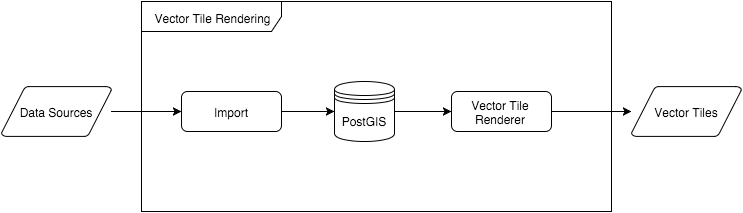
\includegraphics[width=1\textwidth]{images/vector_tile_rendering.png}
  \caption{Vector Tile Rendering Process}
\end{figure}

\section{Tile Server}

To display the rendered vector tiles a tile server and the visual style is needed. There are basically two possibilities, which are described in the following two sections.

\paragraph{Visual Style} \marginpar{A complete specification of what can be defined in the visual style can be found here.\footnote{\url{https://github.com/mapbox/carto/blob/master/docs/latest.md}}}The visual style defines how a feature set such as landuse actually gets displayed. In the case of landuse on could define the texture or the color of the border and area.

\subsection{Raster Tile Server}

The raster tile server makes it possible to display the vector tiles. It takes the visual style and the vector tiles as input. The raster tile renderer generates raster tile of these inputs. When a raster tile is rendered, it gets served by the webserver. Any GIS Software which supports raster tiles could act as a client of our raster tile server.

\begin{figure}[h]

  \centering
  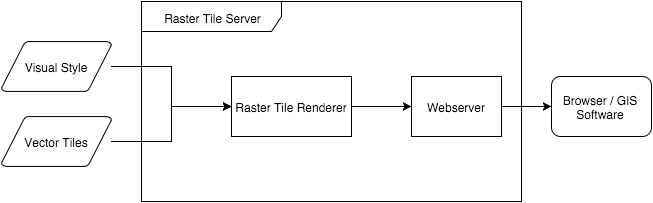
\includegraphics[width=1\textwidth]{images/raster_tile_server.png}
  \caption{Raster tile server}
\end{figure}

\subsection{Vector Tile Server}

The vector tile server in contrast to the raster tile variant directly serves the vector tiles. The raster tiles get rendered on the client side. The advantage of this variant is, that the heavy rendering work is done on the client. 

\begin{figure}[h]

  \centering
  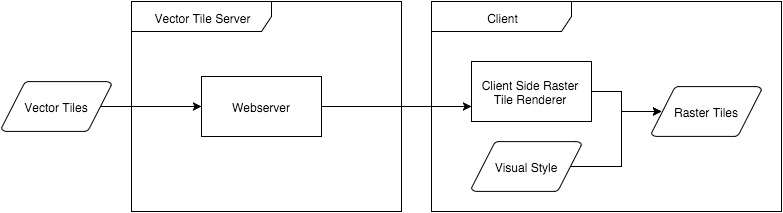
\includegraphics[width=1\textwidth]{images/vector_tile_server.png}
  \caption{Vector tile server}
\end{figure}

\newpage